% !TEX root = main.tex
\section{Specifications}
\label{sec:specifications}
Some key specifications is listed in table \ref{tab:specs_short}. 
% !TEX root = main.tex
% Table generated by Excel2LaTeX from sheet 'specs'
\begin{table}[htbp]
  \centering
  \caption{System specifications}
    \begin{tabular}{lc}
    \rowcolor[rgb]{ 0,  0,  0} \textcolor[rgb]{ 1,  1,  1}{\textbf{System Variables}} & \textcolor[rgb]{ 1,  1,  1}{\textbf{Value}} \\
    \rowcolor[rgb]{ 0,  0,  0} \textcolor[rgb]{ 1,  1,  1}{} & \textcolor[rgb]{ 1,  1,  1}{\textbf{Low / High Data rate}} \\
    Frequency $f_0$ & 2415 MHz \\
    Modulation & QPSK / QAM-64 \\
    Bit per symbol $m$ & 2 /6 \\
    Sound sampling rate $f_s$  & 11025 / 22050 Hz \\
    Bits per sound sample $b_s$ & 8 / 12 bits \\
    Sound datarate $R_{ss}$ & 88,2 / 264,6 kbits/s \\
    Channel coding & Hamming (4,7) \\
    \rowcolor[rgb]{ 0,  0,  0} \textcolor[rgb]{ 1,  1,  1}{\textbf{Transmission Characteristics}} & \textcolor[rgb]{ 1,  1,  1}{} \\
    System bit rate $R_b$ & 191,35 / 577,18 kbits/s \\
    Symbol rate $R_s$ & 95,67 / 96,20 ksymbols/s \\
          &  \\
    Pulse shaping filter & root raised cosine \\
    Pulse shaping filter parameter $\alpha$ & 0.3 \\
    \boldmath{}\textbf{Minimum signal bandwidth $\Delta f$}\unboldmath{} & 62,2 / 62,5 kHz \\
    \end{tabular}%
  \label{tab:specs_short}%
\end{table}%

The values are listed for low / high data rate transmission. The system use the 2.4GHz ISM band with a carrier frequency of 2.415GHz. The system is designed for a transmission distance of 10 meter in an indoor environment with a bandwidth of \bw kHz. 

The adaptable quality is obtained by implementing a feedback path from the receiver to the transmitter. Figure \ref{fig:block_toplevel} shows a top level block diagram of the proposed system. The figure shows that speech data is sent in the forward path from transmitter to receiver, and the number of detected errors is sent in the feedback path from receiver to transmitter. The forward and feedback paths will be referred to as the \textit{data path} and the \textit{BER path} respectively. Block diagrams for these subsystems is shown in appendix \ref{a:block_diagram} and the behaviour will be explained in the following subsection.
% !TEX root = main.tex
\begin{figure}[htbp]
\centering
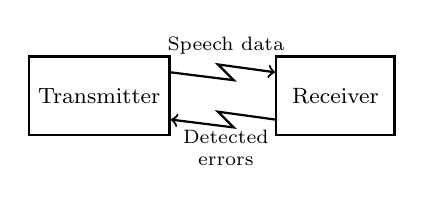
\begin{tikzpicture}[                
                    box/.style={
            		draw,
			thick,
            		text centered,
            		minimum width=1.5cm,
            		minimum height=1cm,
			font=\footnotesize,
			align=center,
			anchor=center,
            	} ]
	

\draw 
(0,0) node[box] (trans) {Transmitter}
(3,0) node[box] (rec) {Receiver}
(rec.west) ++(0,0.3) coordinate[](data_in) {}
(trans.east) ++(0,0.3) coordinate[](data_out) {}
(rec.west) ++(0,-0.3) coordinate[](ber_in) {}
(trans.east) ++(0,-0.3) coordinate[](ber_out) {}
;
\draw[thick, ->] (data_out) -- ++(0.8, -0.1) -- ++(-0.2, 0.2) node[above, align=center, font=\scriptsize, anchor=south, xshift=0.1cm]{Speech data} -- (data_in);
\draw[thick, <-] (ber_out) -- ++(0.8, -0.1) -- ++(-0.2, 0.2) node[below, align=center, font=\scriptsize, anchor=north, yshift=-0.1cm, xshift=0.1cm]{Detected \\ errors} -- (ber_in);

	
\end{tikzpicture}
\caption{Top level block diagram of proposed system. Speech data is sent in the forward path from transmitter to receiver and the number of detected errors is sent back from receiver to transmitter.}
\label{fig:block_toplevel}
\end{figure}

The burst format is shown in figure \ref{fig:burst_format}. 
% !TEX root = main.tex
\begin{figure} 
    \centering
  \subfloat[QPSK data package\label{1a}]{%
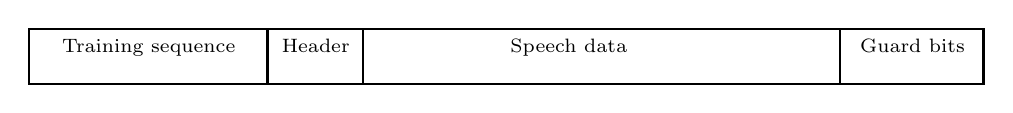
\begin{tikzpicture}[                
                    slot/.style={
            		text centered,
			font=\scriptsize,
			align=center,
			anchor=center,
			minimum height=0.7cm
            	}]
\draw[thick] (0,0) rectangle (\linewidth, -0.7);
\draw[thick] (0.25\linewidth,0) -- ++(0, -0.7);
\draw[thick] (0.35\linewidth,0) -- ++(0, -0.7);
\draw[thick] (0.85\linewidth,0) -- ++(0, -0.7);

\draw
(0,0) node[slot, minimum width=0.25\linewidth, anchor=north west](barker){Training sequence \\ \barkerBitsQPSK}
(0.25\linewidth,0)  node[slot, minimum width=0.1\linewidth, anchor=north west](barker){Header \\ \headerBits}
(0.35\linewidth,0) node[slot, minimum width=0.43\linewidth, anchor=north west](barker){Speech data \\ \packetDataBitsQPSK}
(0.85\linewidth,0) node[slot, minimum width=0.15\linewidth, anchor=north west](barker){Guard bits \\ \guardBitsQPSK}
;	

\end{tikzpicture}
}
  \\
  \subfloat[QAM-64 data package\label{1b}]{%
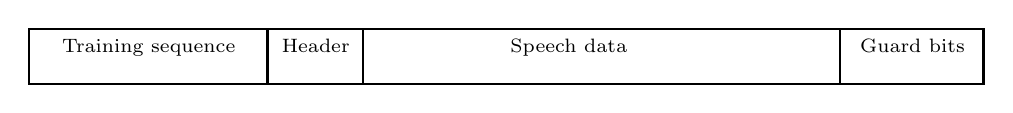
\begin{tikzpicture}[                
                    slot/.style={
            		text centered,
			font=\scriptsize,
			align=center,
			anchor=center,
			minimum height=0.7cm
            	}]
\draw[thick] (0,0) rectangle (\linewidth, -0.7);
\draw[thick] (0.25\linewidth,0) -- ++(0, -0.7);
\draw[thick] (0.35\linewidth,0) -- ++(0, -0.7);
\draw[thick] (0.85\linewidth,0) -- ++(0, -0.7);

\draw
(0,0) node[slot, minimum width=0.25\linewidth, anchor=north west](barker){Training sequence \\ \barkerBitsQAM}
(0.25\linewidth,0)  node[slot, minimum width=0.1\linewidth, anchor=north west](barker){Header \\ \headerBits}
(0.35\linewidth,0) node[slot, minimum width=0.43\linewidth, anchor=north west](barker){Speech data \\ \packetDataBitsQAM}
(0.85\linewidth,0) node[slot, minimum width=0.15\linewidth, anchor=north west](barker){Guard bits \\ \guardBitsQAM}
;	

\end{tikzpicture}}
\\
  \subfloat[QPSK BER package\label{1c}]{%
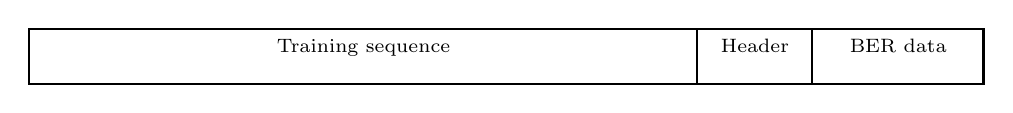
\begin{tikzpicture}[                
                    slot/.style={
            		text centered,
			font=\scriptsize,
			align=center,
			anchor=center,
			minimum height=0.7cm
            	}]
\draw[thick] (0,0) rectangle (\linewidth, -0.7);
\draw[thick] (0.70\linewidth,0) -- ++(0, -0.7);
\draw[thick] (0.82\linewidth,0) -- ++(0, -0.7);

\draw
(0,0) node[slot, minimum width=0.7\linewidth, anchor=north west](barker){Training sequence \\ \barkerBitsQPSK}
(0.70\linewidth,0)  node[slot, minimum width=0.12\linewidth, anchor=north west](barker){Header \\ \headerBits}
(0.82\linewidth,0) node[slot, minimum width=0.18\linewidth, anchor=north west](barker){BER data \\ \BERDataBits}
;	

\end{tikzpicture}}
  \caption{Burst format for QPSK(a) and QAM-64(b) modulated data bursts, and QPSK modulated BER burst (c)}
  \label{fig:burst_format} 
\end{figure}


\subsection{Sound Producer and Sound Consumer}
The blocks sound producer and sound consumer contains functionality for handling the sound input and output to the sound card of the computer. Sound producer reads sound samples at from the sound card at full quality, i.e. 16 bit, 44100 Hz stereo, and writes the samples to a queue accessible for the source encoder. Sound consumer equivalently reads sound samples from a queue controlled by the unpacking block and writes to the computer sound card.

\subsection{Source Encoder}
The source encoder performs lossy compression of the produced sound samples. The samples produced by sound producer are stored as 64 bit unsigned integers (u64) even though the resolution is only 16 bits. This means that the 48 least significant bits of each sample is zero. Depending on the state of the system (High or low quality transmission) the source encoder read several u64s and pack them into one single u64. Five or eight samples are packed into each u64 depending on the state (see details in table \ref{tab:specs}). In addition the sample rate are reduced by decimation with a factor of 2 or 4 for high and low quality respectively. 

\subsection{Packing}
Add header and write to packet queue. Need more info.

\subsection{Forward Error Correction}
The implemented FEC algorithm is Hamming (7,4). The implementation is a very fast, pre-written C-code.

\subsection{Symbol Mapping}
The system uses Grey Code for symbol mapping 


